\documentclass[t]{beamer}

% Load general definitions
% Preamble file - general definitions, package loading, etc.

%=================================
% Load packages
\usepackage{amssymb,amsmath}
\usepackage{graphicx}
\usepackage{url}
\usepackage{tikz}
\usetikzlibrary{mindmap,trees,arrows}
\usepackage{fancyvrb}
\usepackage[portuguese]{babel} 
\usepackage[utf8]{inputenc}
\usepackage{subfigure}
\usepackage{times}
\usepackage[T1]{fontenc}
\usepackage{cancel}
\usepackage{color}
\usepackage{listings}
\usepackage[document]{ragged2e}

%=================================
% Set mode
\mode<presentation>
{
	\usetheme{Madrid}
	\usecolortheme{structure}
	\useoutertheme{infolines}
	\setbeamercovered{invisible}
}

% Get rid of nav bar
\beamertemplatenavigationsymbolsempty

% Insert frame number at bottom of the page.
\usefoottemplate{\hfil\tiny{\color{black!90}\insertframenumber}} 

%=================================
% Define new commands

\newcommand\Real{{\mathbb{R}}}
%\newcommand{\vi}{\vspace{0.6\baselineskip}}
%\newcommand{\goodgap}{\hspace{\subfigtopskip}\hspace{\subfigbottomskip}}


% Equation environments
\newcommand{\beq}{\begin{equation}}
\newcommand{\eq}{\end{equation}}
\newcommand{\beqs}{\begin{equation*}}
\newcommand{\eqs}{\end{equation*}}
\newcommand{\beqn}{\begin{eqnarray}}
\newcommand{\eqn}{\end{eqnarray}}
% Bold variables
\newcommand{\mbf}[1]{\ensuremath{\mathbf{#1}}}
% Itemization
\newcommand{\bitem}{\begin{itemize}}
\newcommand{\eitem}{\end{itemize}}
\newcommand{\spitem}{\vskip 1em\item}
\newcommand{\bitems}{\begin{itemize}\item}
\newcommand{\benums}{\begin{enumerate}\item}
\newcommand{\eenum}{\end{enumerate}}
% color blocks
\newenvironment{colorblock}[2]{%
\setbeamercolor{block title}{#2}
\begin{block}{#1}}{\end{block}}
% Vertical spacing
\newcommand{\vone}{\vskip 1em}
\newcommand{\vhalf}{\vskip .5em}
% Frame environments
\newenvironment{ftst}[3][t]{%
\begin{frame}{environment=ftst,#1}
\frametitle{#2}
\framesubtitle{#3}}{\end{frame}}
\newenvironment{ftstf}[2]{
\begin{frame}[fragile,environment=ftstf]
\frametitle{#1}
\framesubtitle{#2}}{\end{frame}}
% colors
\definecolor{MyGray}{rgb}{0.5,0.5,0.5}
\definecolor{MyDBGray}{rgb}{0.1,0.1,0.4}
\definecolor{darkgreen}{rgb}{0,0.4,0}
\definecolor{black}{rgb}{0,0,0}
\def\defn#1{{\color{red} #1}}
% Footnote
\renewcommand{\thefootnote}{\alph{footnote}}
% Relaxed footnotes
\newcommand{\lfr}[1]{\let\thefootnote\relax\footnote{\tiny #1}}
% Verbatim environment - using FANCYVRB package
\DefineVerbatimEnvironment%
{rcode}{Verbatim}
{fontsize=\scriptsize}
% Verbatim environment - using LISTINGS package
%\lstnewenvironment{rcode} {\lstset{	language = R,
%									basicstyle = \scriptsize\ttfamily,
%									showspaces = false,
%									showstringspaces = false,
%									showtabs = false,
%									keywordstyle = \color{black}\bfseries,
%									commentstyle = \color{darkgreen},
%									numbers = none,
%									otherkeywords={	<-,
%													ggplot,
%													geom_boxplot,
%													facet_grid,
%													shapiro.test,
%													fligner.test,
%													glht,
%													with},
%									deletekeywords={data,
%													model,
%													residuals,
%													c,
%													axis,
%													default,
%													labels,
%													qq.text}}}%
%{}

% Specific definitions
\title[]{Pesquisa Operacional}
\subtitle[]{Introdução à Pesquisa Operacional}
\author[]{Patrícia Lucas\\{\footnotesize }}
\institute{Bacharelado em Sistemas de Informação \\ IFNMG  - Campus Salinas}
\date{\scriptsize Salinas\\Dezembro 2021}

\begin{document}

% cover page
\setbeamertemplate{footline}{}
\begin{frame}

\begin{center}
\includegraphics[width=.15\textwidth]{}
\end{center}
  \titlepage
  \begin{tikzpicture}[remember picture,overlay]
  \node[anchor=south east,xshift=-5pt,yshift=5pt] at (current page.south east) {\tiny Versão 1.2021};
  \node[anchor=south west,yshift=0pt] at (current page.south west) {
\includegraphics[width=.25\textwidth]{Logos/salinas_horizontal_jpg.jpg}};
  \end{tikzpicture}  
\end{frame}

% Main slides
%==================================


\begin{ftst}{Visão geral}{Introdução à Pesquisa Operacional}
\small
\begin{itemize}
    \item A Pesquisa Operacional, ou simplesmente PO, surgiu na Inglaterra durante a Segunda Guerra Mundial (1939-1945) para a solução de problemas de natureza logística, tática e de estratégia militar, marcando a primeira atividade formal desse campo de estudo. 
    \vone
    \item Os resultados positivos alcançados fizeram com que a Pesquisa Operacional fosse disseminada nos Estados Unidos e, em 1947, a equipe liderada por George B. Dantzig deu origem ao método Simplex para resolução de problemas de programação linear.
    \vone
    \item Desde então, esse conhecimento vem sendo aplicado, com sucesso, para a otimização de recursos em diversos segmentos industriais e comerciais de várias áreas de negócio (estratégia, marketing, finanças, microeconomia, operações e logística, recursos humanos, entre outras).
\end{itemize}

\end{ftst}

%==================================

\begin{ftst}{Visão geral}{Introdução à Pesquisa Operacional}
\begin{itemize}
    \item O avanço da Pesquisa Operacional tornou-se possível graças ao aumento da velocidade de processamento e à quantidade de memória de computadores nos últimos anos, tornando possível a solução de problemas complexos. 
    \vone
    \item Um profissional de PO deve ser capaz de identificar a técnica mais apropriada para a solução de determinado tipo de problema, os objetivos para a melhoria, as limitações físicas e computacionais do sistema, sendo o elemento humano fundamental nesse processo.
\end{itemize}

\end{ftst}

%==================================

\begin{ftst}{Visão geral}{Introdução à Pesquisa Operacional}
\begin{itemize}
    \item Em termos gerais, podemos dizer que a Pesquisa Operacional consiste na utilização de um método científico (modelos matemáticos, estatísticos e algoritmos computacionais) para a tomada de decisões.
    \vone
    \item Dessa forma, a PO atua cada vez mais em um ramo multidisciplinar, envolvendo áreas de engenharia de produção, matemática aplicada, ciência da computação e gestão de negócios.
\end{itemize}
\end{ftst}

%==================================

\begin{ftst}{O processo de tomada de decisão}{Introdução à Pesquisa Operacional}
\begin{itemize}
    \item \textbf{Decisão:} o processo de análise entre várias alternativas disponíveis do curso de ação que a pessoa deverá seguir.
    \item \textbf{Tomada de decisão:} o processo pelo qual são escolhidas algumas ou apenas uma entre muitas alternativas para as ações a serem realizadas.
    \item \textbf{Exemplo:} a escolha de uma alternativa de localização dentre várias disponíveis.
\end{itemize}

\end{ftst}

%==================================

\begin{ftst}{O processo de tomada de decisão}{Introdução à Pesquisa Operacional}
\begin{itemize}
    \item A tomada de decisões é um processo complexo e envolve diversos fatores internos e externos ligados à organização:
    \begin{figure}
        \centering
        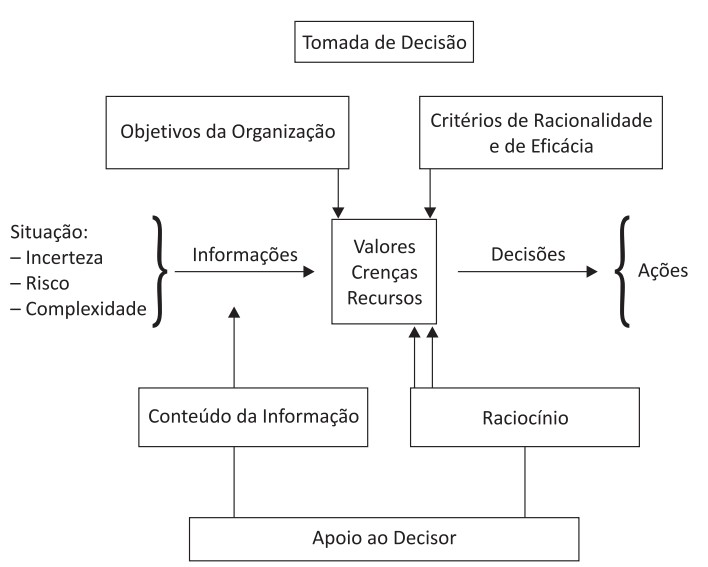
\includegraphics[scale=0.4]{Figuras/tomada_decisao.jpg}
    \end{figure}
\end{itemize}

\end{ftst}

%==================================

\begin{ftst}{O processo de tomada de decisão}{Introdução à Pesquisa Operacional}
\small
\begin{itemize}
    \item Ainda existem profissionais e executivos de mercado que insistem em tomar suas decisões sem qualquer embasamento proveniente de um tratamento de dados e sem a consideração de incertezas, riscos e complexidades inerentes ao processo.
    \item O correto tratamento e a adequada análise dos dados podem propiciar, ao tomador de decisão, informações mais precisas e confiáveis que, quando confrontadas com outras informações ou submetidas a provas existentes e a restrições impostas pelo sistema, oferecem o diferencial do conhecimento.
    \begin{figure}
        \centering
        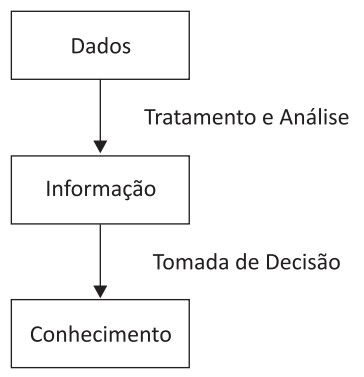
\includegraphics[scale=0.3]{Figuras/conhecimento.jpg}
    \end{figure}
    \end{itemize}

\end{ftst}

%==================================

\begin{ftst}{Modelagem para Tomada de Decisão}{Introdução à Pesquisa Operacional}
\small
\begin{itemize}
    \item Um modelo é a representação simplificada de um sistema real, podendo ser um projeto já existente ou um projeto futuro.
    \vone
    \item No primeiro caso, pretende-se reproduzir o funcionamento do sistema real existente, de forma a aumentar a produtividade, enquanto no segundo caso o objetivo é definir a estrutura ideal do futuro sistema. 
    \vone
    \item O comportamento de um sistema real é influenciado por diversas variáveis envolvidas no processo de tomada de decisão. Devido à grande complexidade desse sistema, torna-se necessária a sua simplificação, a partir de um modelo, de forma que as principais variáveis envolvidas no sistema ou projeto que se pretende entender ou controlar sejam consideradas na sua construção.
\end{itemize}

\end{ftst}

%==================================

\begin{ftst}{Modelagem para Tomada de Decisão}{Introdução à Pesquisa Operacional}

\begin{itemize}
    \item Um modelo é composto por três elementos principais: 
    \vone
    \begin{itemize}
        \item[a.] Variáveis de Decisão e Parâmetros;
        \vone
        \item[b.] Função Objetivo;
        \vone
        \item[c.] Restrições.
    \end{itemize}
    
\end{itemize}

\end{ftst}

%==================================

\begin{ftst}{Modelagem para Tomada de Decisão}{Introdução à Pesquisa Operacional}
\small
\begin{itemize}
    \item[\textbf{a.}] \textbf{Variáveis de Decisão: }são as incógnitas, ou valores desconhecidos, que serão determinados pela solução do modelo. Representam efetivamente a decisão que deve ser tomada no problema modelado.
    
    \item  \textbf{Escalas de mensuração:}
    \begin{itemize}
        \footnotesize
        \item As variáveis \textbf{contínuas} podem assumir quaisquer valores em um intervalo de números reais (conjunto infinito ou não enumerável de valores). Exemplo: quantidade ótima a ser produzida (em litros) de cada tipo de refrigerante em uma empresa de bebidas.
        \item As variáveis \textbf{discretas} podem assumir valores dentro de um conjunto finito ou uma quantidade enumerável de valores, sendo aquelas provenientes de determinada contagem. Exemplo:  número ideal de funcionários por turno de trabalho.
        \item As variáveis \textbf{binárias} podem assumir dois possíveis valores: 1 (quando a característica de interesse está presente na variável) ou 0 (caso contrário). Exemplo: fabricar ou não determinado produto.
    \end{itemize}
\end{itemize}

\end{ftst}

%==================================

\begin{ftst}{Modelagem para Tomada de Decisão}{Introdução à Pesquisa Operacional}
\small
\begin{itemize}
    \item[\textbf{b.}] \textbf{Parâmetros:} são os valores fixos previamente conhecidos do problema.
    \vone
    \item Exemplo: custo por funcionário contratado.
\end{itemize}

\end{ftst}

%==================================

\begin{ftst}{Modelagem para Tomada de Decisão}{Introdução à Pesquisa Operacional}

\begin{itemize}
    \item[\textbf{d.}] \textbf{Função Objetivo:} é uma função matemática que determina o valor-alvo que se pretende alcançar ou a qualidade da solução, em função das variáveis de decisão e dos parâmetros, podendo ser uma função de \textit{maximização} ou de \textit{minimização}.
    \vone
    \item Exemplo: minimização do custo total de produção de diversos tipos de chocolates, maximização do lucro líquido na fabricação de diversos tipos de refrigerantes.
\end{itemize}

\end{ftst}

%==================================

\begin{ftst}{Modelagem para Tomada de Decisão}{Introdução à Pesquisa Operacional}

\begin{itemize}
    \item[\textbf{c.}] \textbf{Restrições:} são um conjunto de equações (expressões matemáticas de igualdade) e inequações (expressões matemáticas de desigualdade) que as variáveis de decisão do modelo devem satisfazer. 
    \vone
    \item As restrições são adicionadas ao modelo de forma a considerar as limitações físicas do sistema, e afetam diretamente os valores das variáveis de decisão. 
    \vone
    \item Exemplo: capacidade máxima de produção, demanda mínima aceitável de um produto.
\end{itemize}

\end{ftst}

%==================================

\begin{ftst}{Modelagem para Tomada de Decisão}{Introdução à Pesquisa Operacional}

\textbf{Exemplo:} Ache o máximo da função $f(x_1,x_2) = x_1 + x_2$, supondo que $x_1$ e $x_2$ satisfaçam:
\begin{equation*}
    \left\{\begin{matrix}
        x_1 \geq 0
        \\ x_2 \geq 0
        \\ 2x_1 + x_2 \leq 4
        \\ x_1 + 2x_2 \leq 3
\end{matrix}\right.
\end{equation*}
\vone
Quais são as variáveis de decisão? 
\vone
Qual é a função objetivo? 
\vone
Esse problema é restrito ou irrestrito? 
\vone
Se restrito, quais são as restrições?

\end{ftst}

%==================================

\begin{ftst}{Classificação das ferramentas da PO}{Introdução à Pesquisa Operacional}
\begin{itemize}
    \item Os modelos determinísticos são aqueles em que todas as variáveis envolvida em sua formulação são constantes e conhecidas. Os modelos determinísticos são frequentemente resolvidos por métodos analíticos (sistema de equações) que geram a solução ótima.
\end{itemize}

\begin{figure}
    \centering
    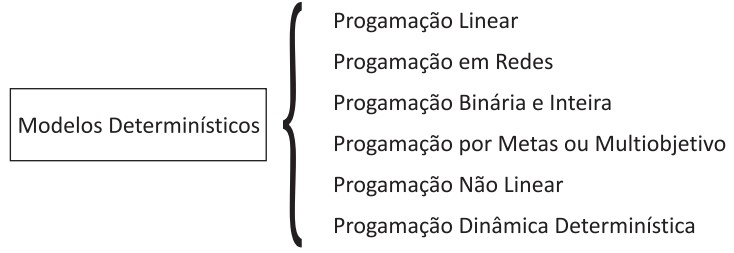
\includegraphics[scale=0.5]{Figuras/deterministicos.jpg}
\end{figure}
\end{ftst}

%==================================

\begin{ftst}{Classificação das ferramentas da PO}{Introdução à Pesquisa Operacional}
\begin{itemize}
    \item Os modelos estocásticos utilizam uma ou mais variáveis aleatórias em que pelo menos uma de suas características operacionais é definida por meio de funções de probabilidade. Dessa forma, os modelos estocásticos geram mais de uma solução e buscam analisar os diferentes cenários, não tendo a garantia da solução ótima.
\end{itemize}

\begin{figure}
    \centering
    \includegraphics[scale=0.5]{Figuras/estocásticos.jpg}
\end{figure}
\end{ftst}

%==================================

\begin{ftst}{Classificação das ferramentas da PO}{Introdução à Pesquisa Operacional}

\begin{figure}
    \centering
    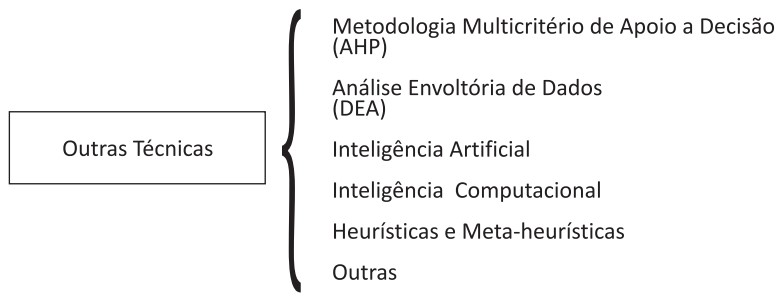
\includegraphics[scale=0.5]{Figuras/outras_tecnicas.jpg}
\end{figure}
\end{ftst}

%==================================

\end{document}

